\section{Resultados}


\begin{frame}
     \begin{figure}
         \scalebox{0.60}{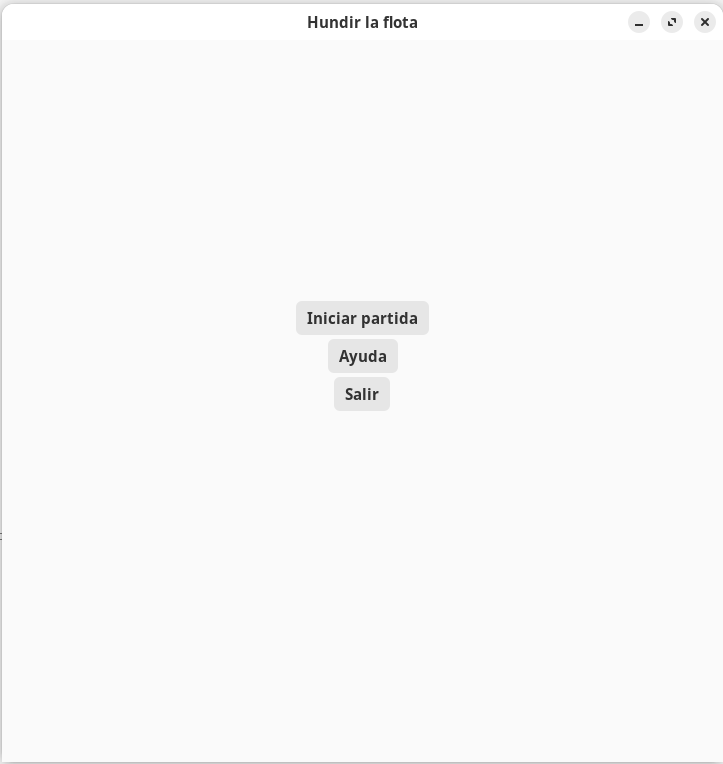
\includegraphics[width = \textwidth]{imagenes/resultados/inicio.png}}
         \caption{Menú de inicio de la aplicación}
       \end{figure}
\end{frame}

\begin{frame}
    \begin{columns}
        \column{\dimexpr\paperwidth-10pt}
        \begin{figure}
            \scalebox{1}{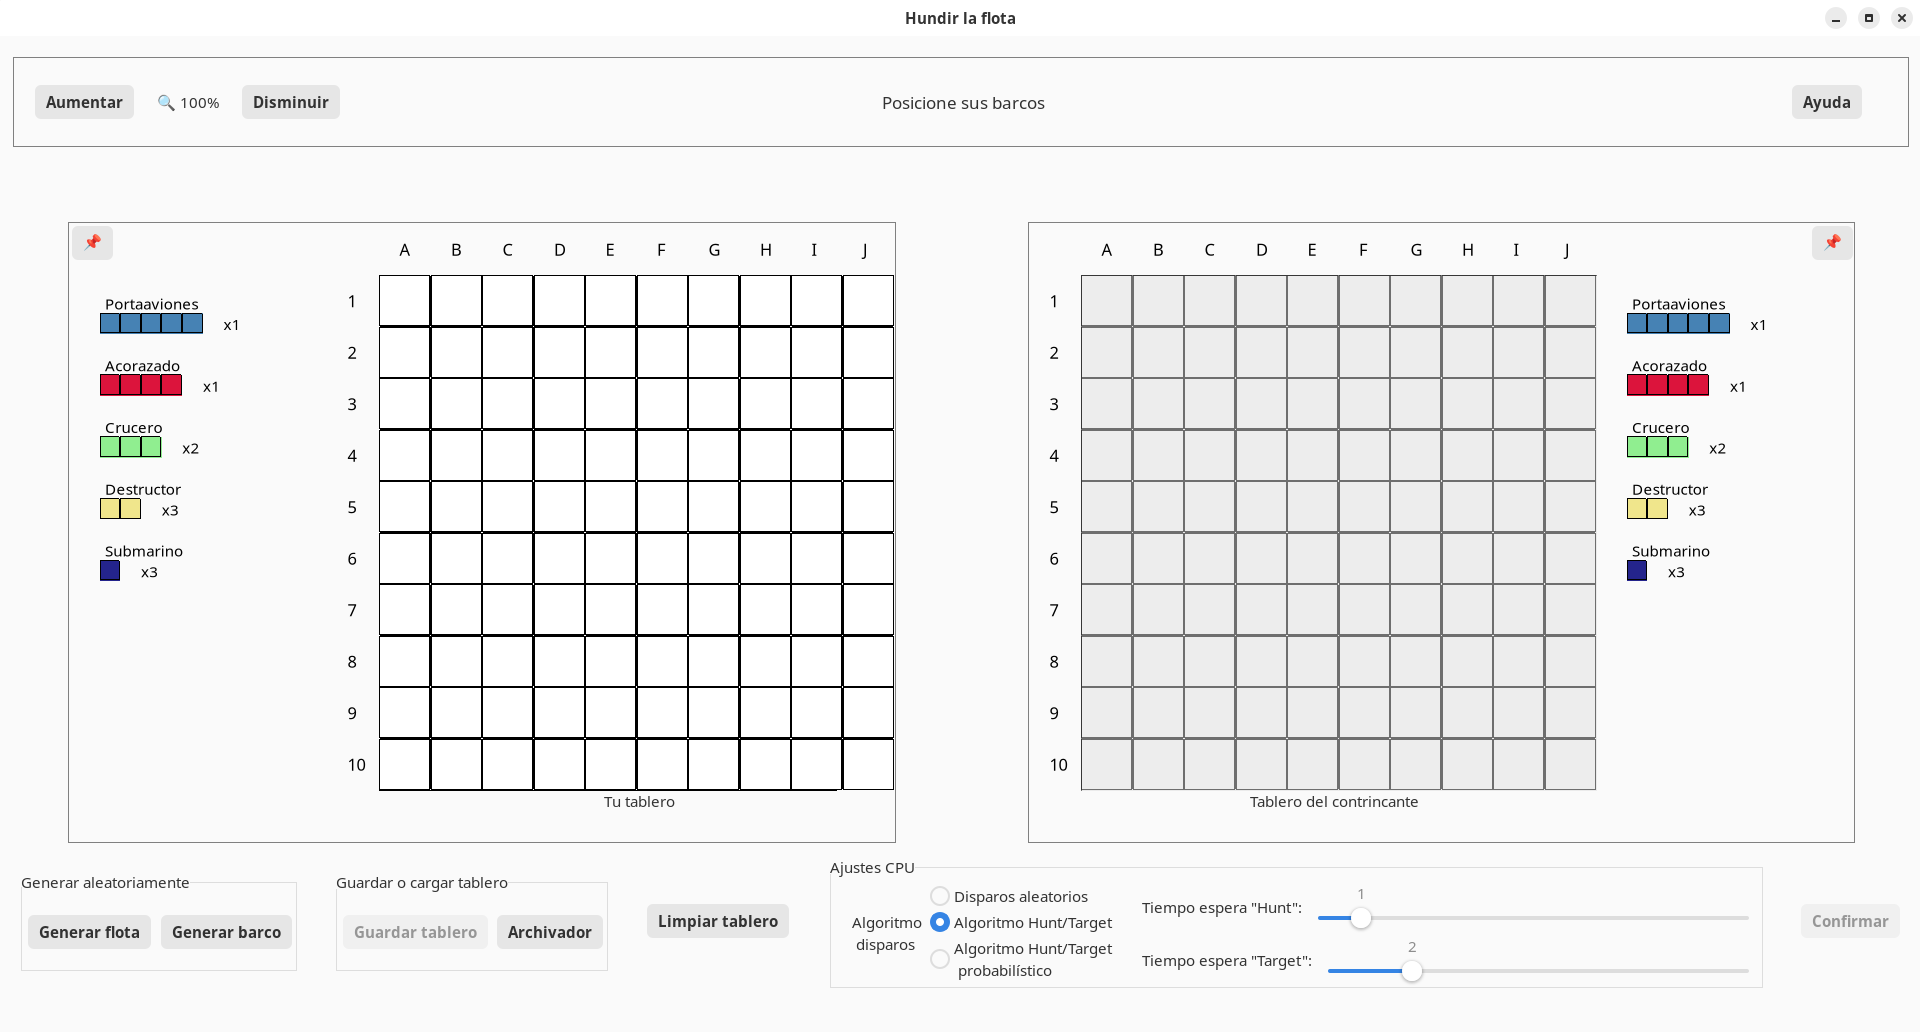
\includegraphics[width = \textwidth]{imagenes/resultados/principal.png}}
            \caption{Pantalla principal de la aplicación}
          \end{figure}
      \end{columns}
\end{frame}

\begin{frame}
    \begin{columns}
        \column{\dimexpr\paperwidth-10pt}
        \begin{figure}
            \scalebox{1}{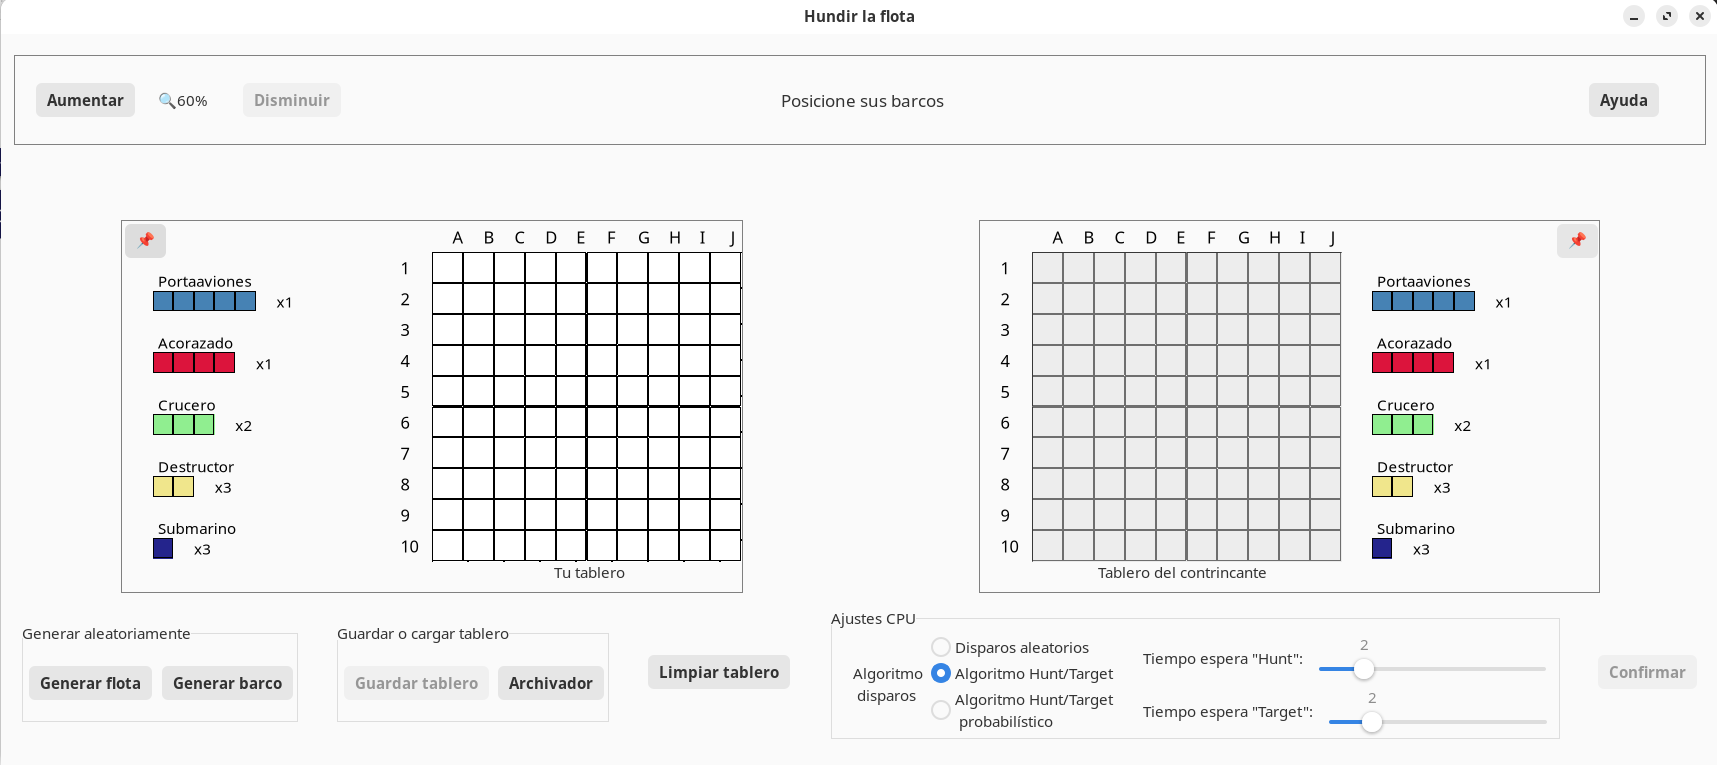
\includegraphics[width = \textwidth]{imagenes/resultados/disminuir.png}}
            \caption{Disminuir el tamaño de la interfaz}
          \end{figure}
      \end{columns}
\end{frame}

\begin{frame}
    \begin{columns}
        \column{\dimexpr\paperwidth-10pt}
        \begin{figure}
            \scalebox{1}{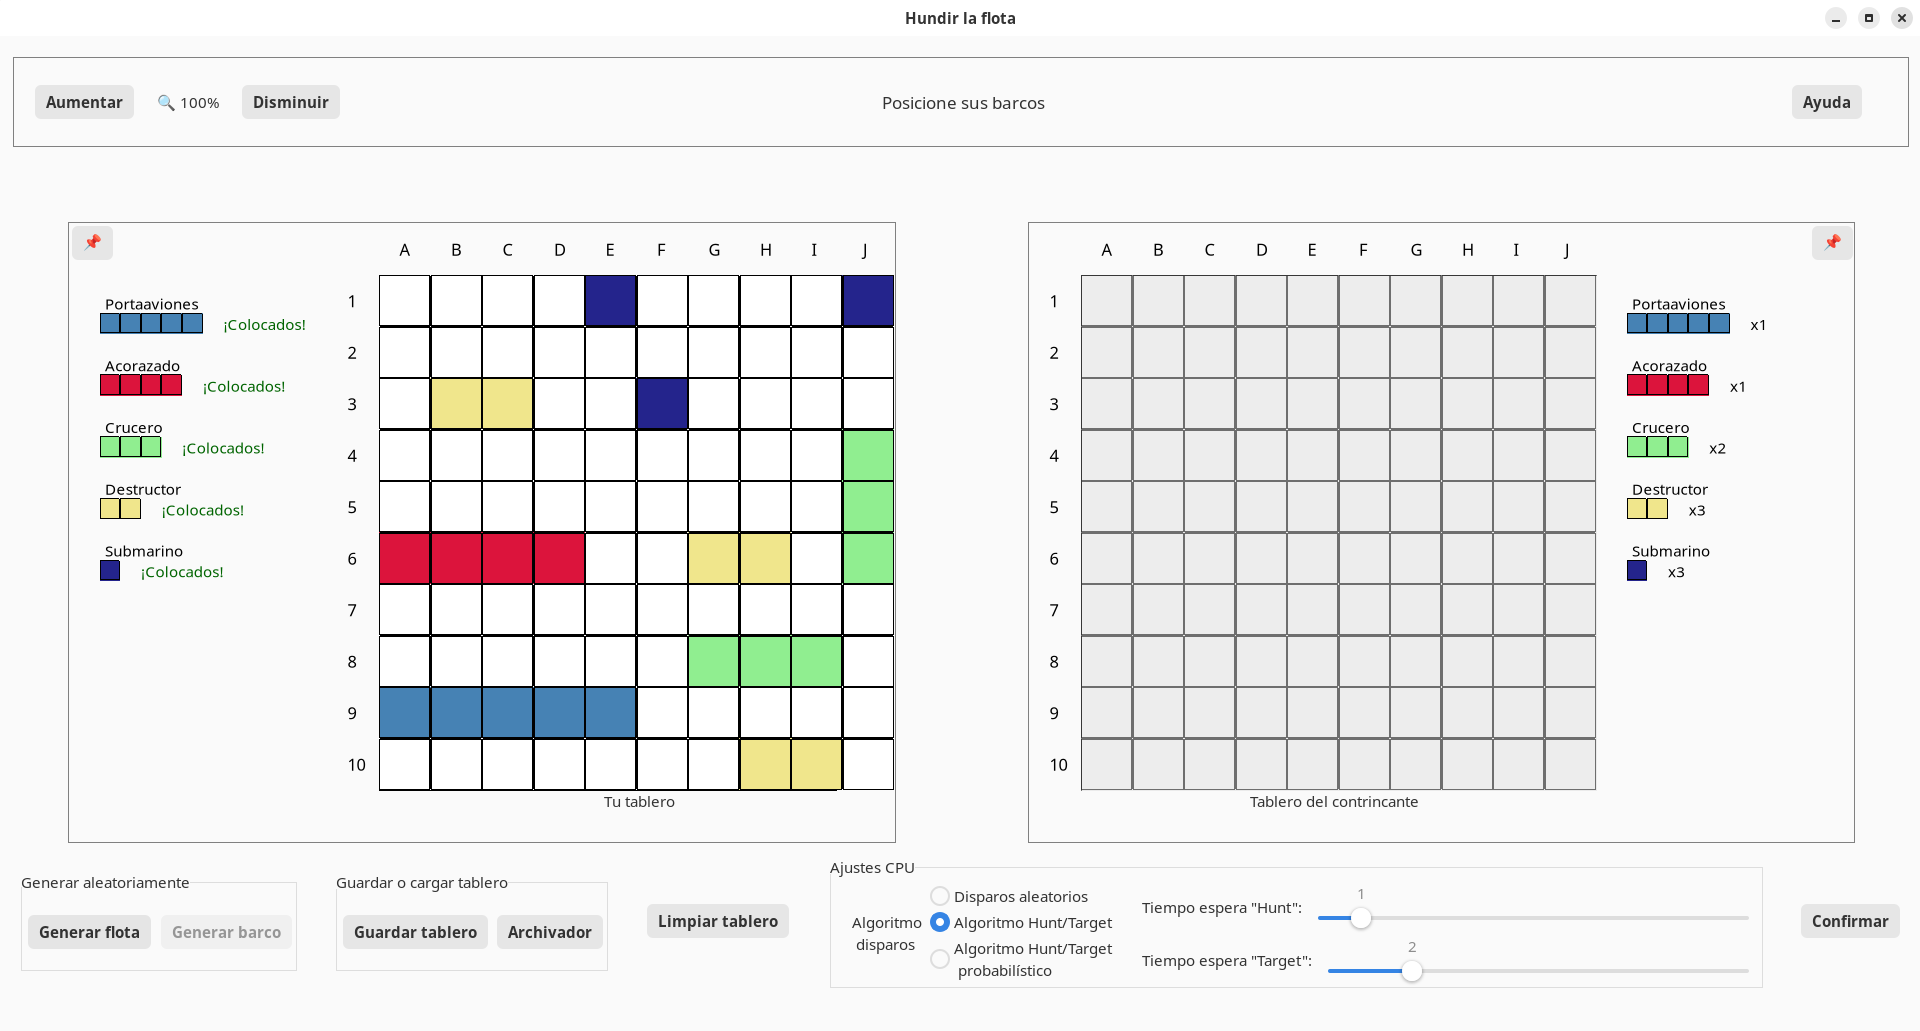
\includegraphics[width = \textwidth]{imagenes/resultados/colocacionAleatoria.png}}
            \caption{Ejemplo de colocación de los barcos aleatoria}
          \end{figure}
      \end{columns} 
\end{frame}

\begin{frame}
    \begin{columns}
        \column{\dimexpr\paperwidth-10pt}
        \begin{figure}
            \scalebox{1}{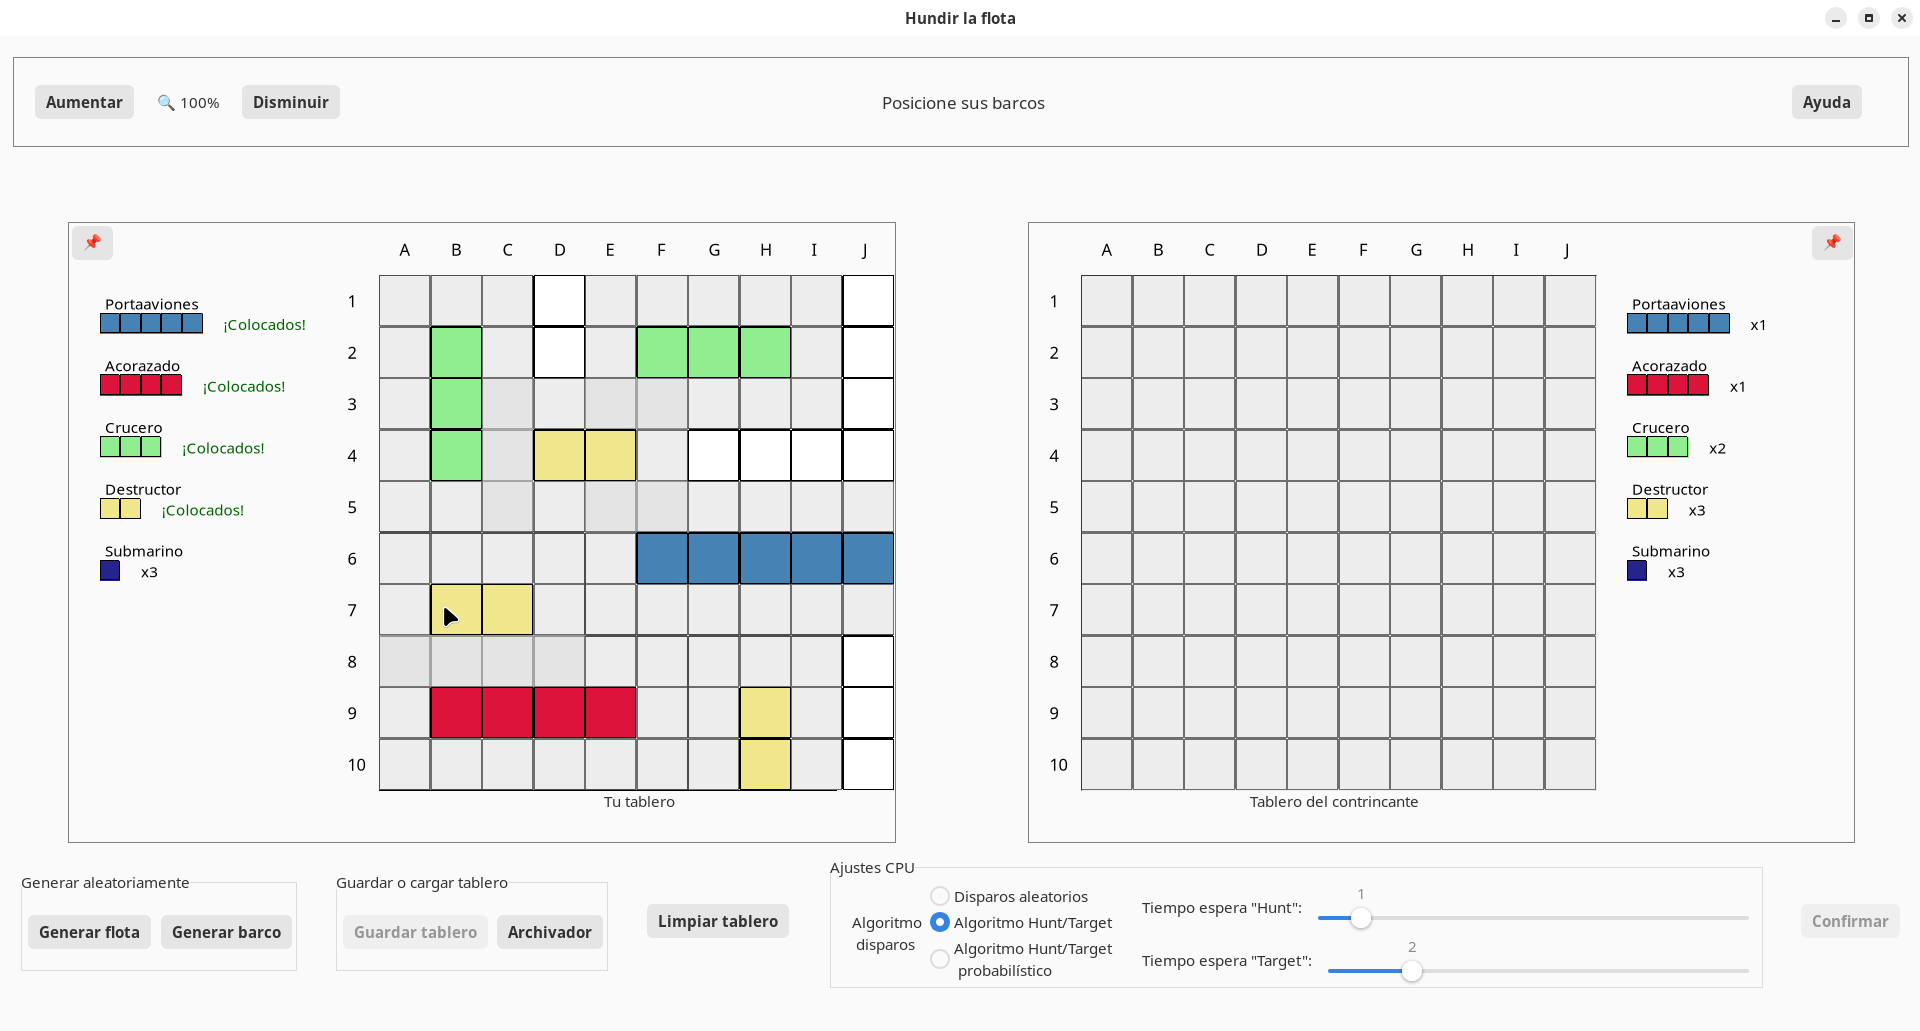
\includegraphics[width = \textwidth]{imagenes/resultados/colocacionManual.png}}
            \caption{Ejemplo de colocación de los barcos manual}
          \end{figure}
      \end{columns}   
\end{frame}


\begin{frame}
    \begin{columns}
        \column{\dimexpr\paperwidth-10pt}
        \begin{figure}
            \scalebox{1}{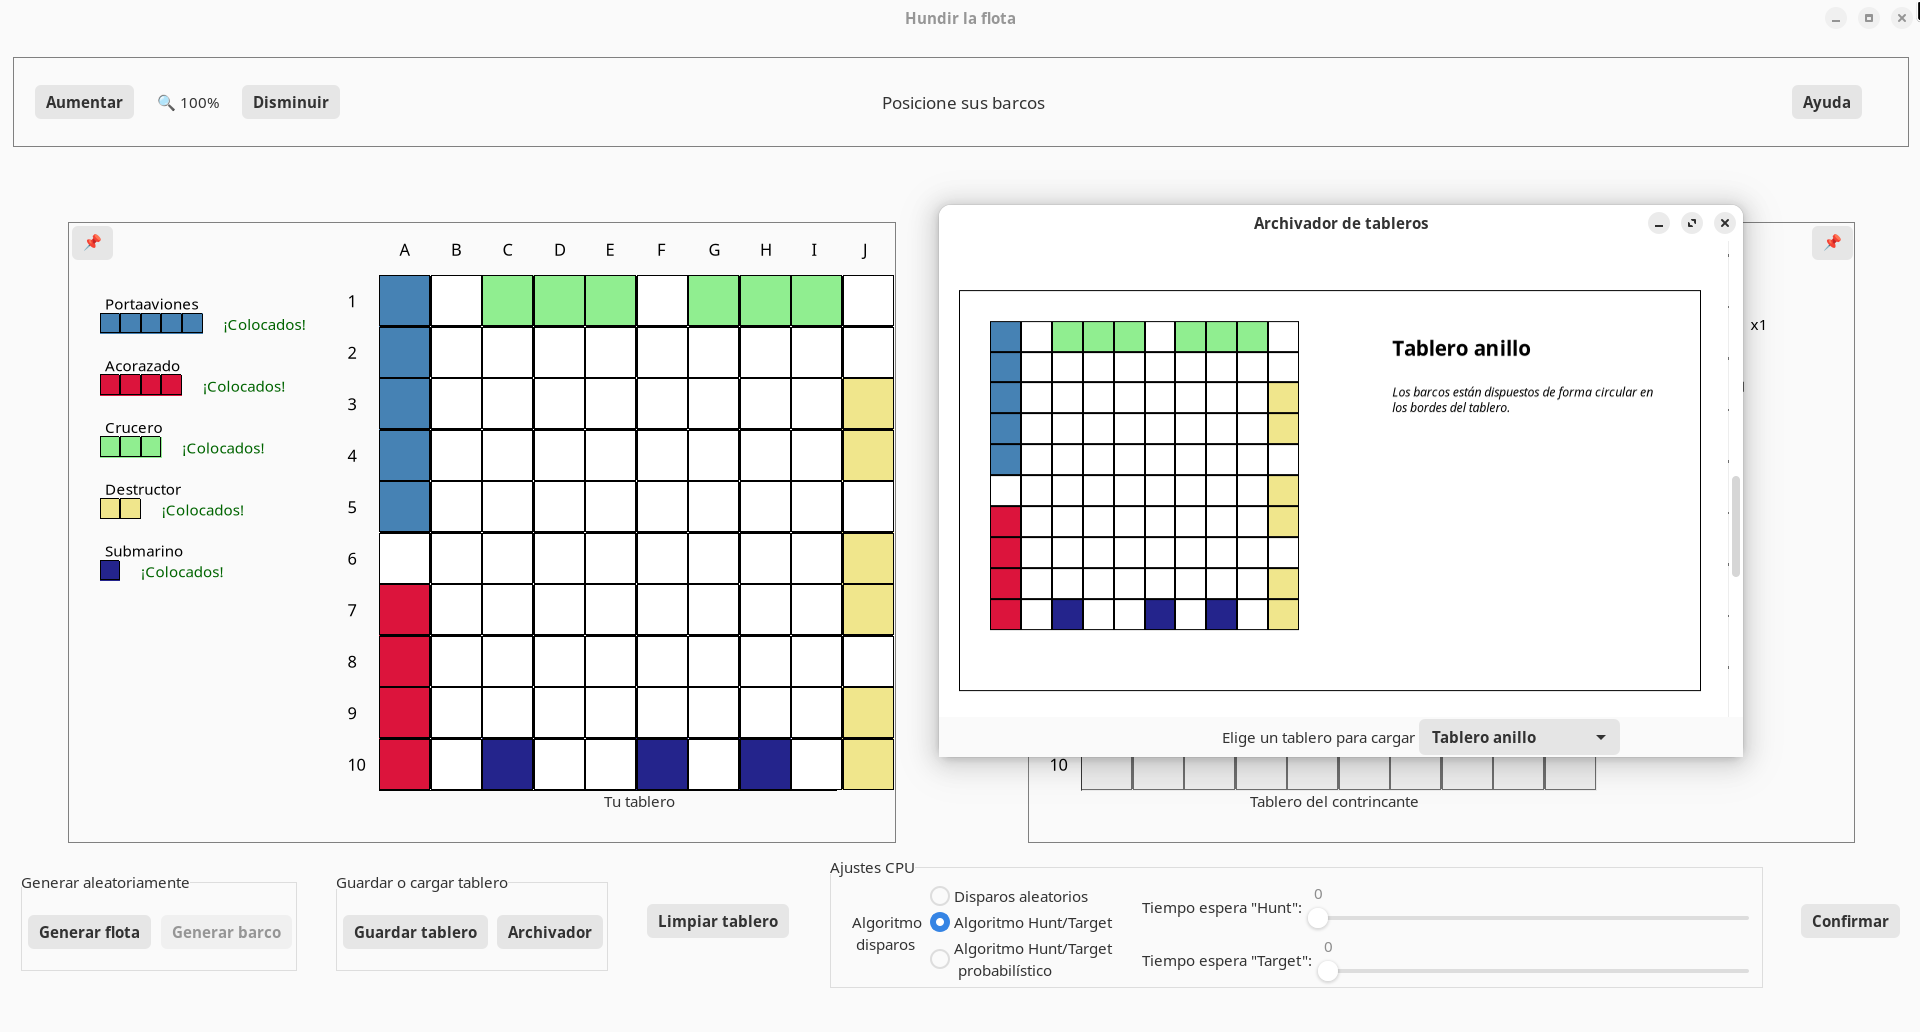
\includegraphics[width = \textwidth]{imagenes/resultados/cargar.png}}
            \caption{Uso del archivador}
          \end{figure}
      \end{columns}
\end{frame}

\begin{frame}
    \begin{columns}
        \column{\dimexpr\paperwidth-10pt}
        \begin{figure}
            \scalebox{1}{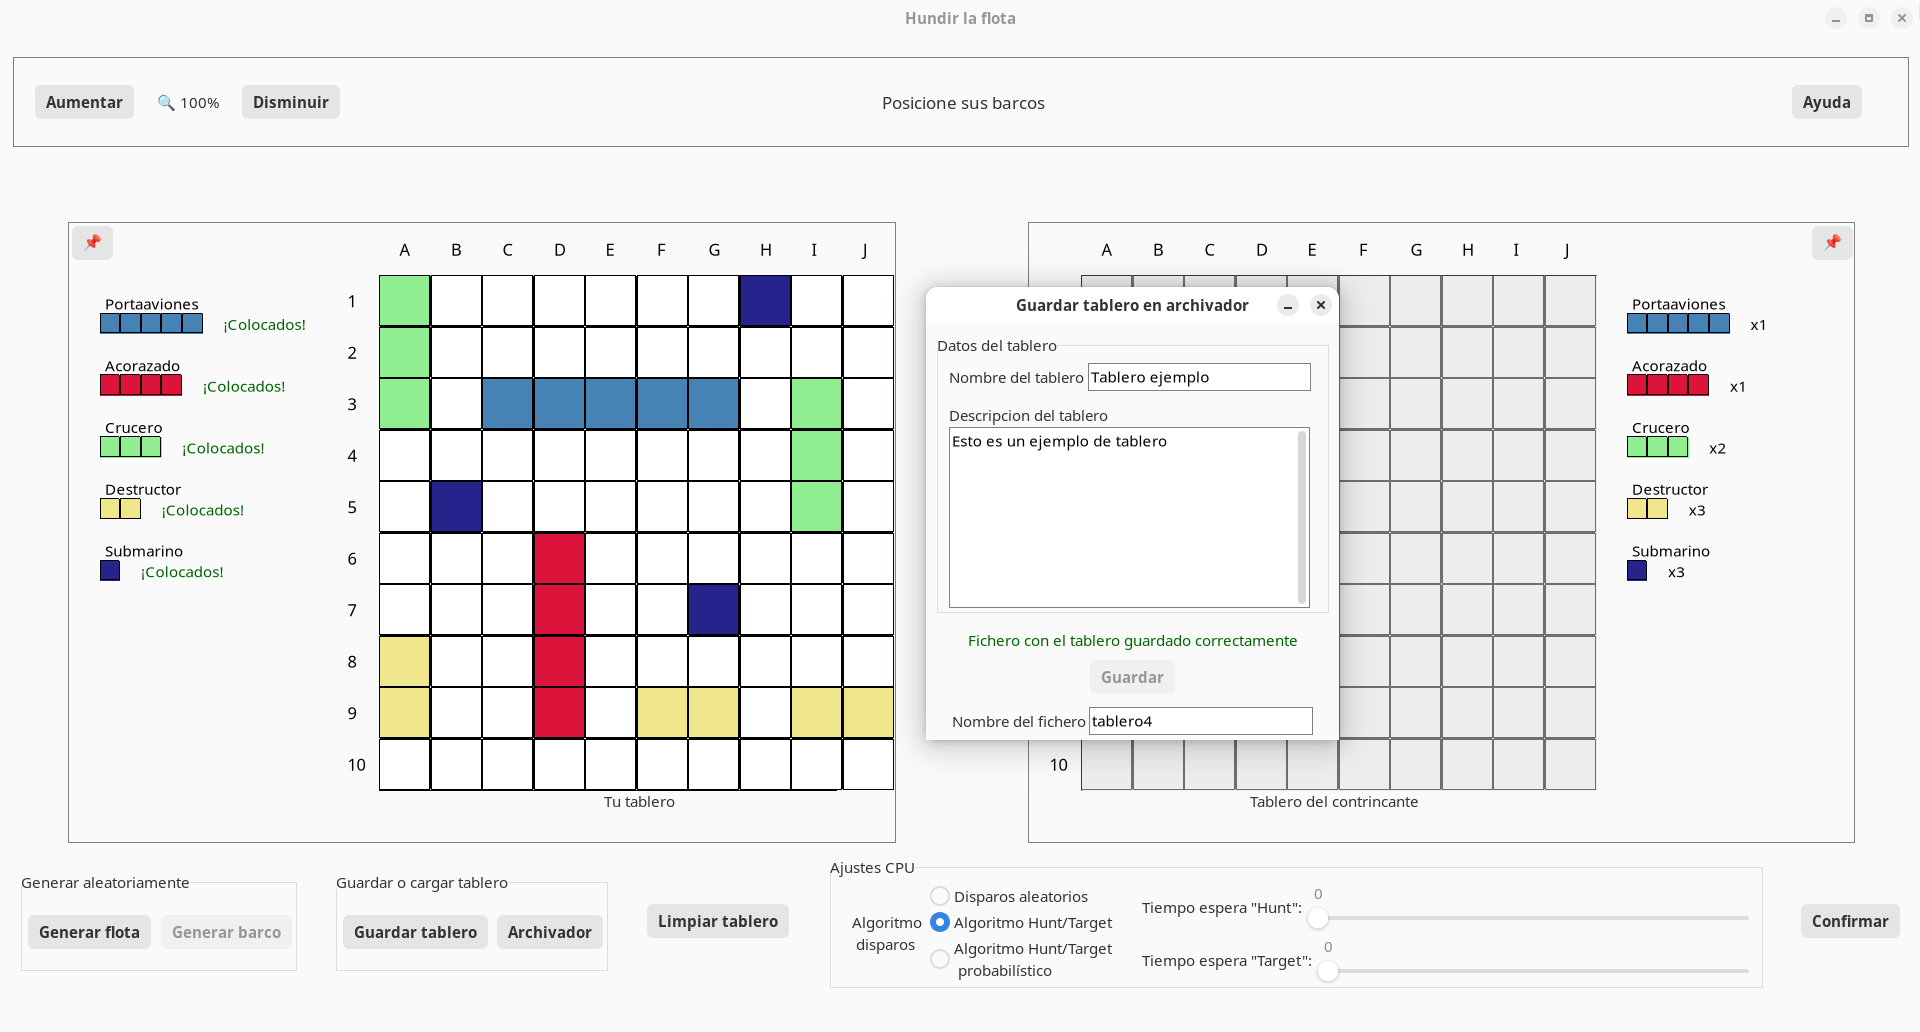
\includegraphics[width = \textwidth]{imagenes/resultados/guardar.png}}
            \caption{Guardar un tablero en el archivador}
          \end{figure}
      \end{columns}
\end{frame}

\begin{frame}
    \begin{columns}
        \column{\dimexpr\paperwidth-10pt}
        \begin{figure}
            \scalebox{1}{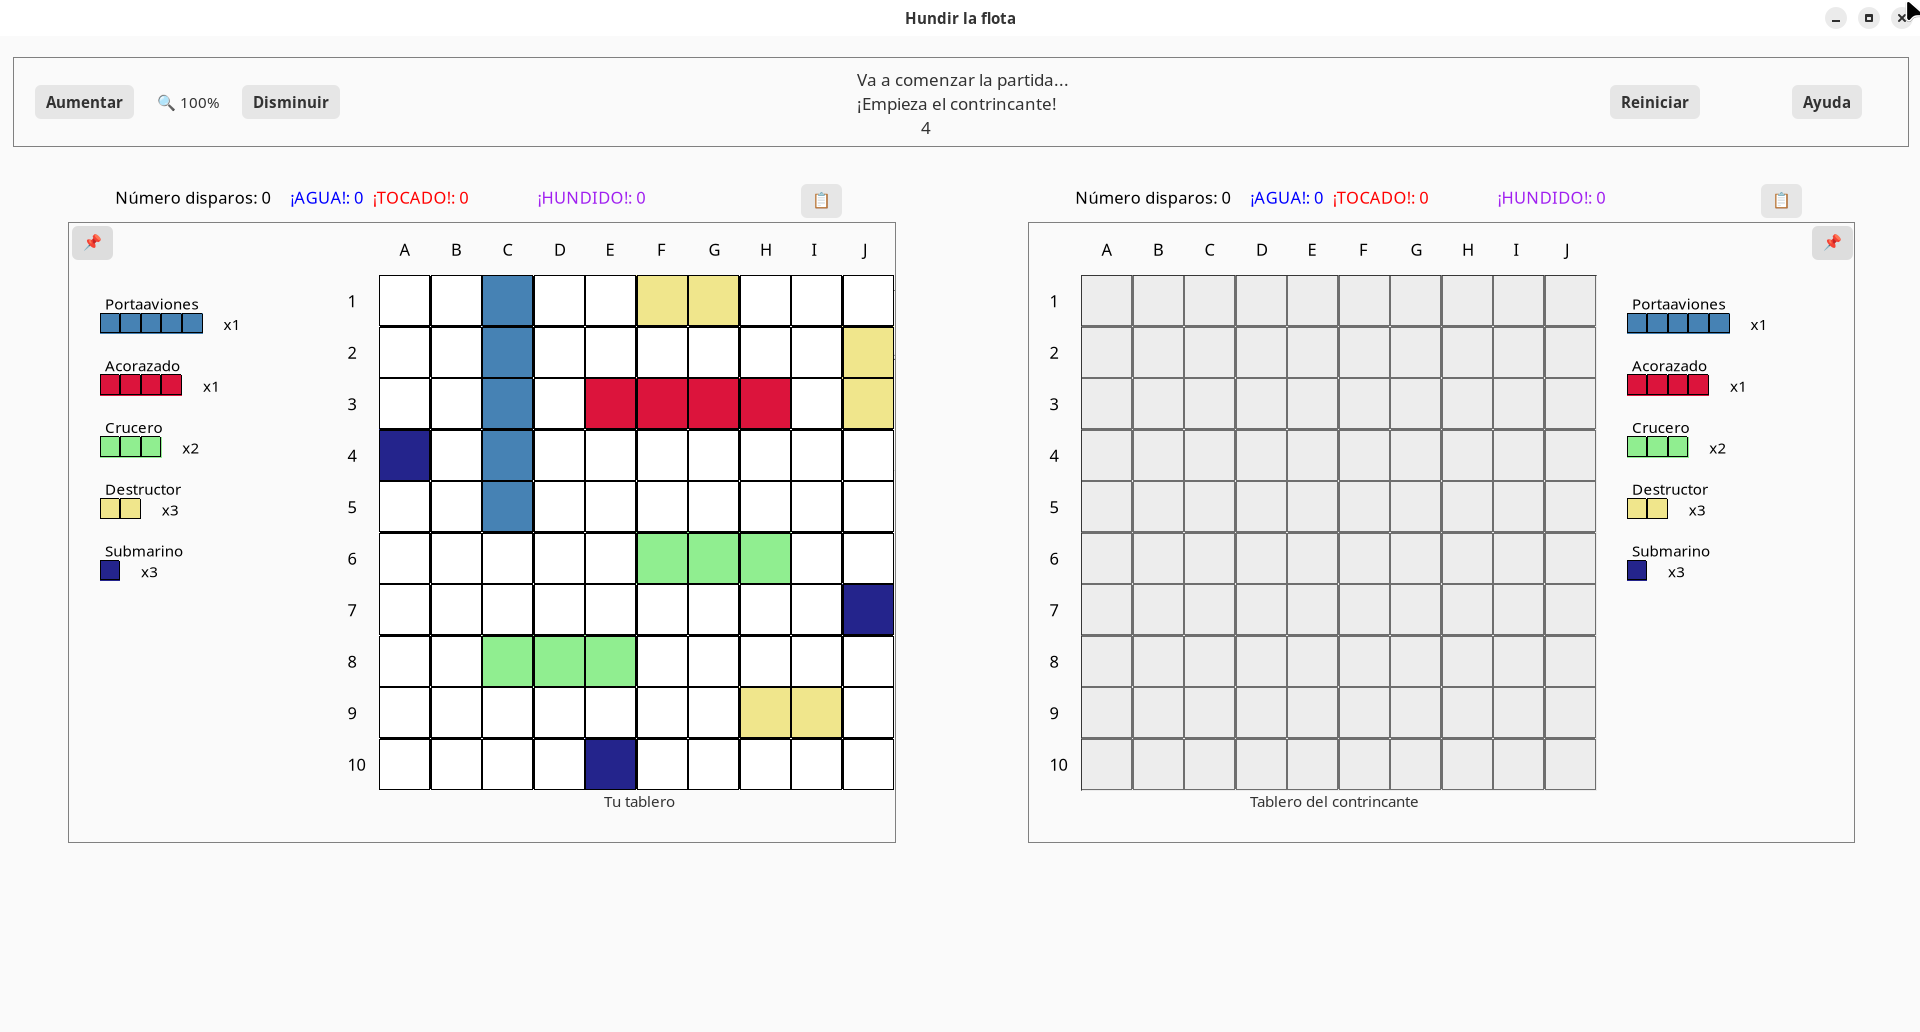
\includegraphics[width = \textwidth]{imagenes/resultados/partida.png}}
            \caption{Inicio de partida}
          \end{figure}
      \end{columns}
\end{frame}

\begin{frame}
    \begin{columns}
        \column{\dimexpr\paperwidth-10pt}
        \begin{figure}
            \scalebox{1}{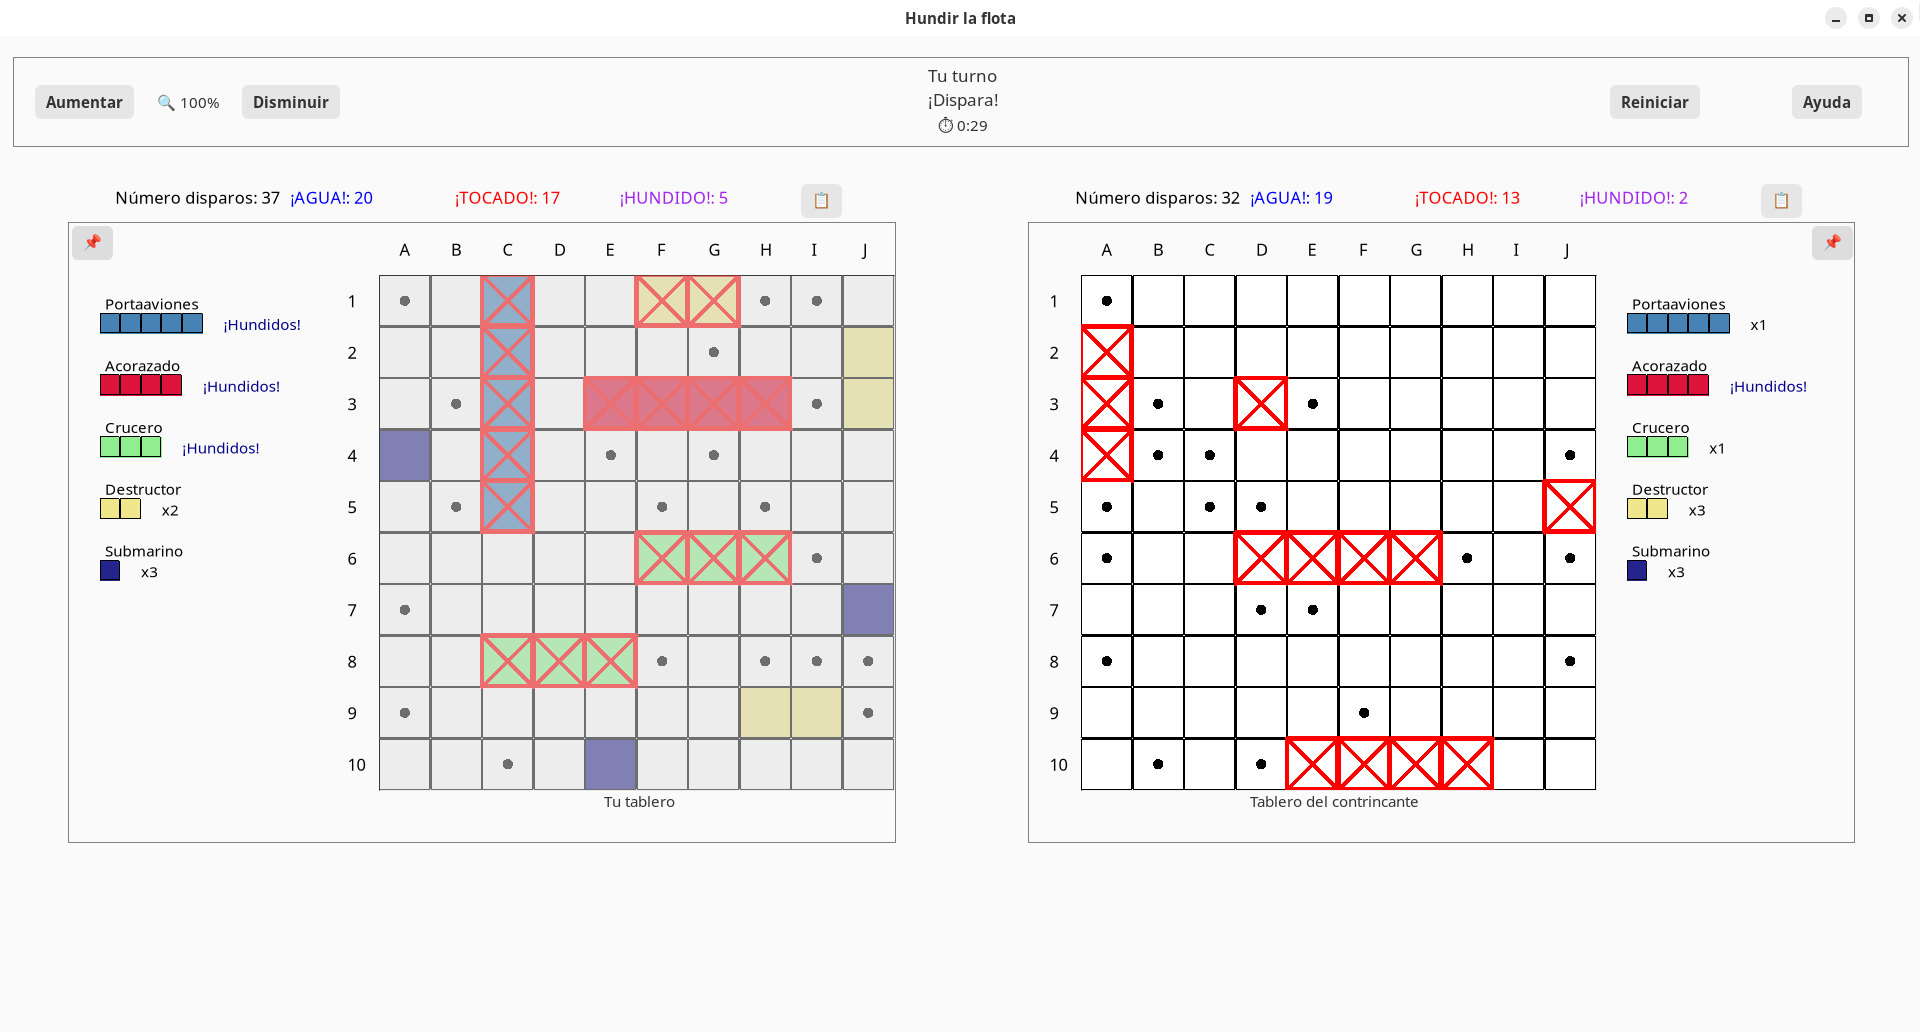
\includegraphics[width = \textwidth]{imagenes/resultados/turnoJugador.png}}
            \caption{Turno del jugador}
          \end{figure}
      \end{columns}
\end{frame}

\begin{frame}
    \begin{columns}
        \column{\dimexpr\paperwidth-10pt}
        \begin{figure}
            \scalebox{1}{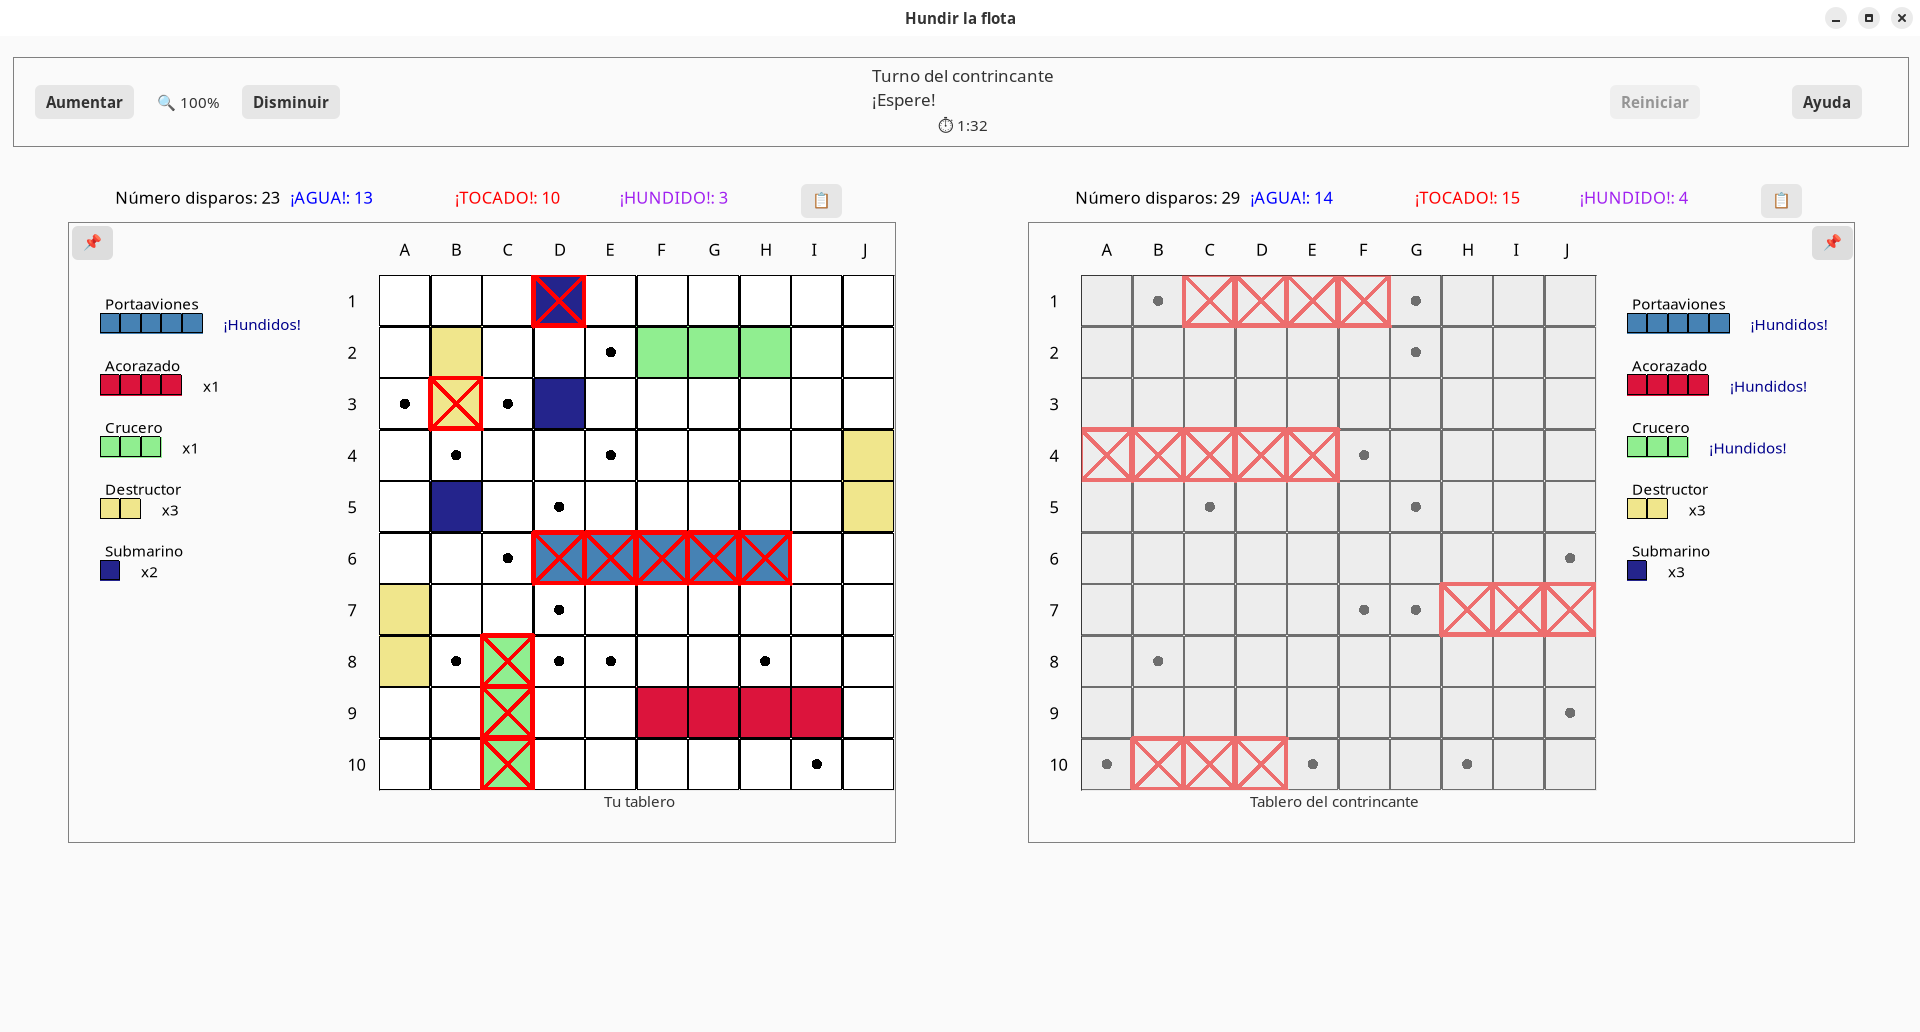
\includegraphics[width = \textwidth]{imagenes/resultados/turnoCPU.png}}
            \caption{Turno de la máquina (\textit{CPU})}
          \end{figure}
      \end{columns}
\end{frame}


\begin{frame}
    \begin{columns}
        \column{\dimexpr\paperwidth-10pt}
        \begin{figure}
            \scalebox{1}{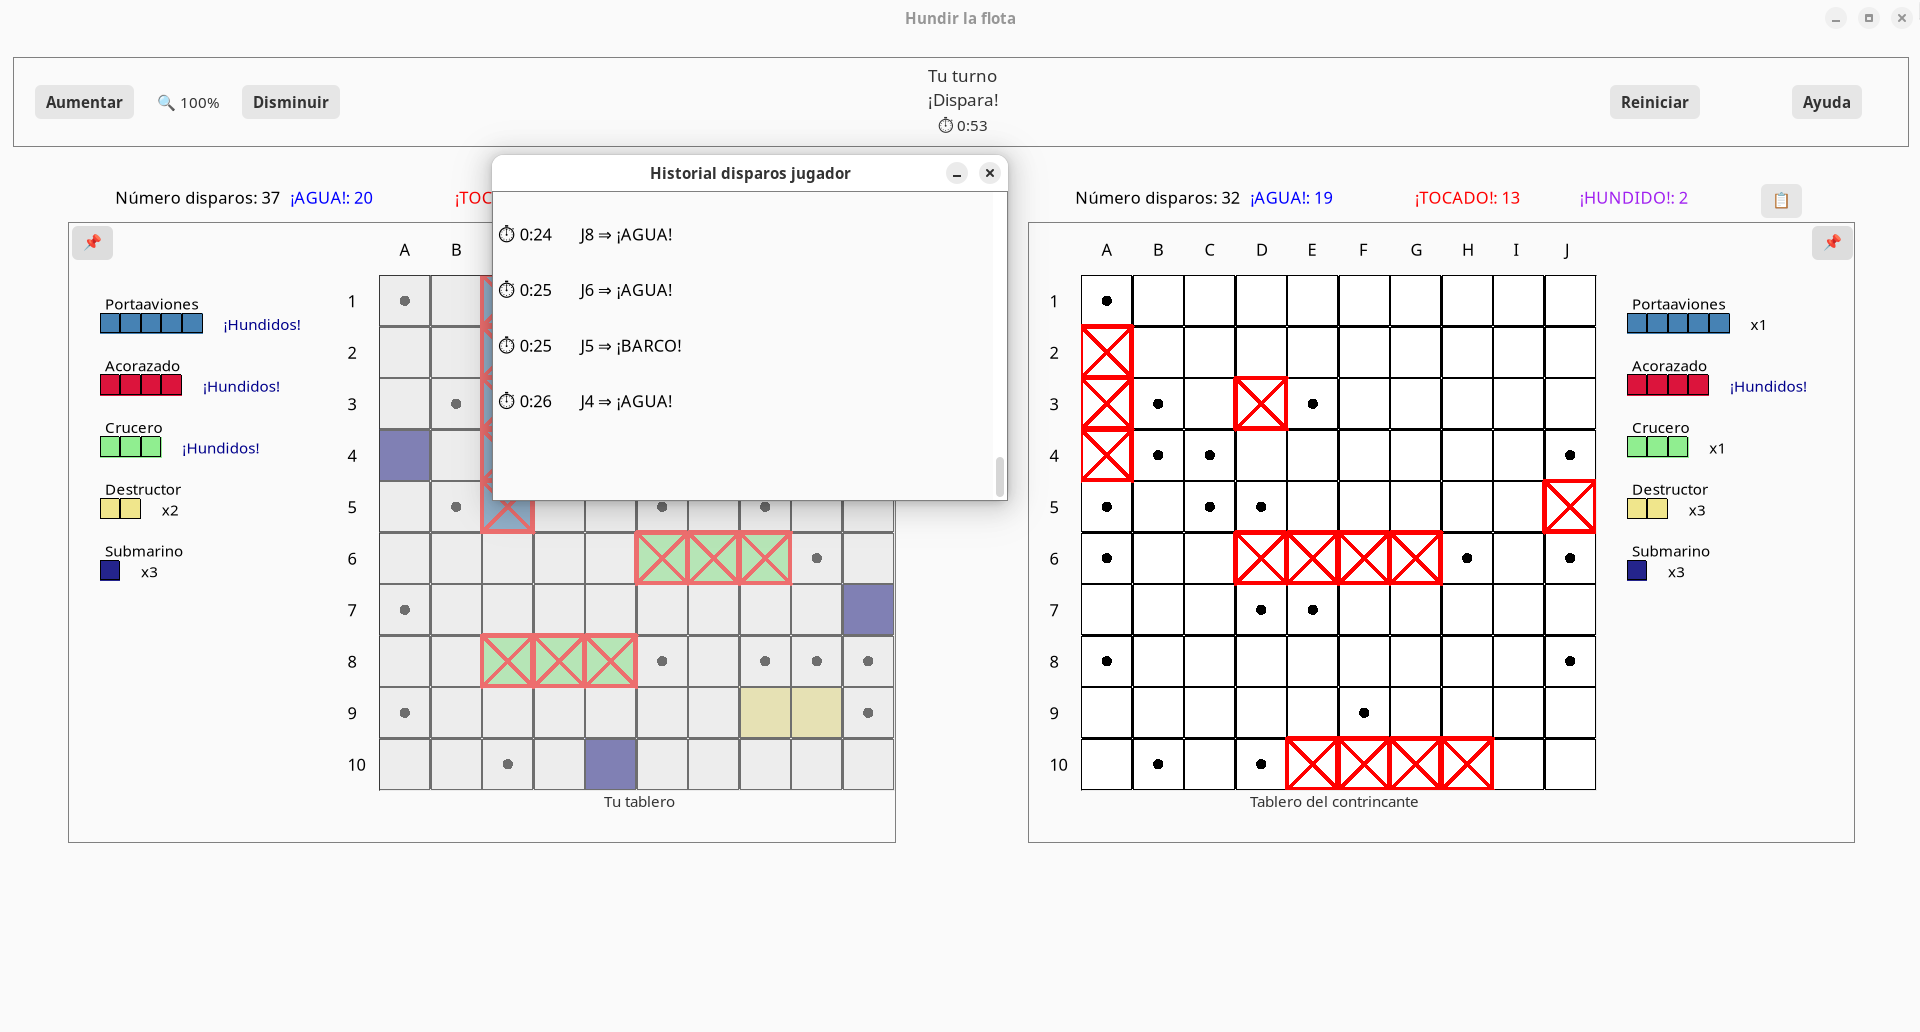
\includegraphics[width = \textwidth]{imagenes/resultados/historial.png}}
            \caption{Uso del historial de disparos}
          \end{figure}
      \end{columns}
\end{frame}


\begin{frame}
    \begin{columns}
        \column{\dimexpr\paperwidth-10pt}
        \begin{figure}
            \scalebox{1}{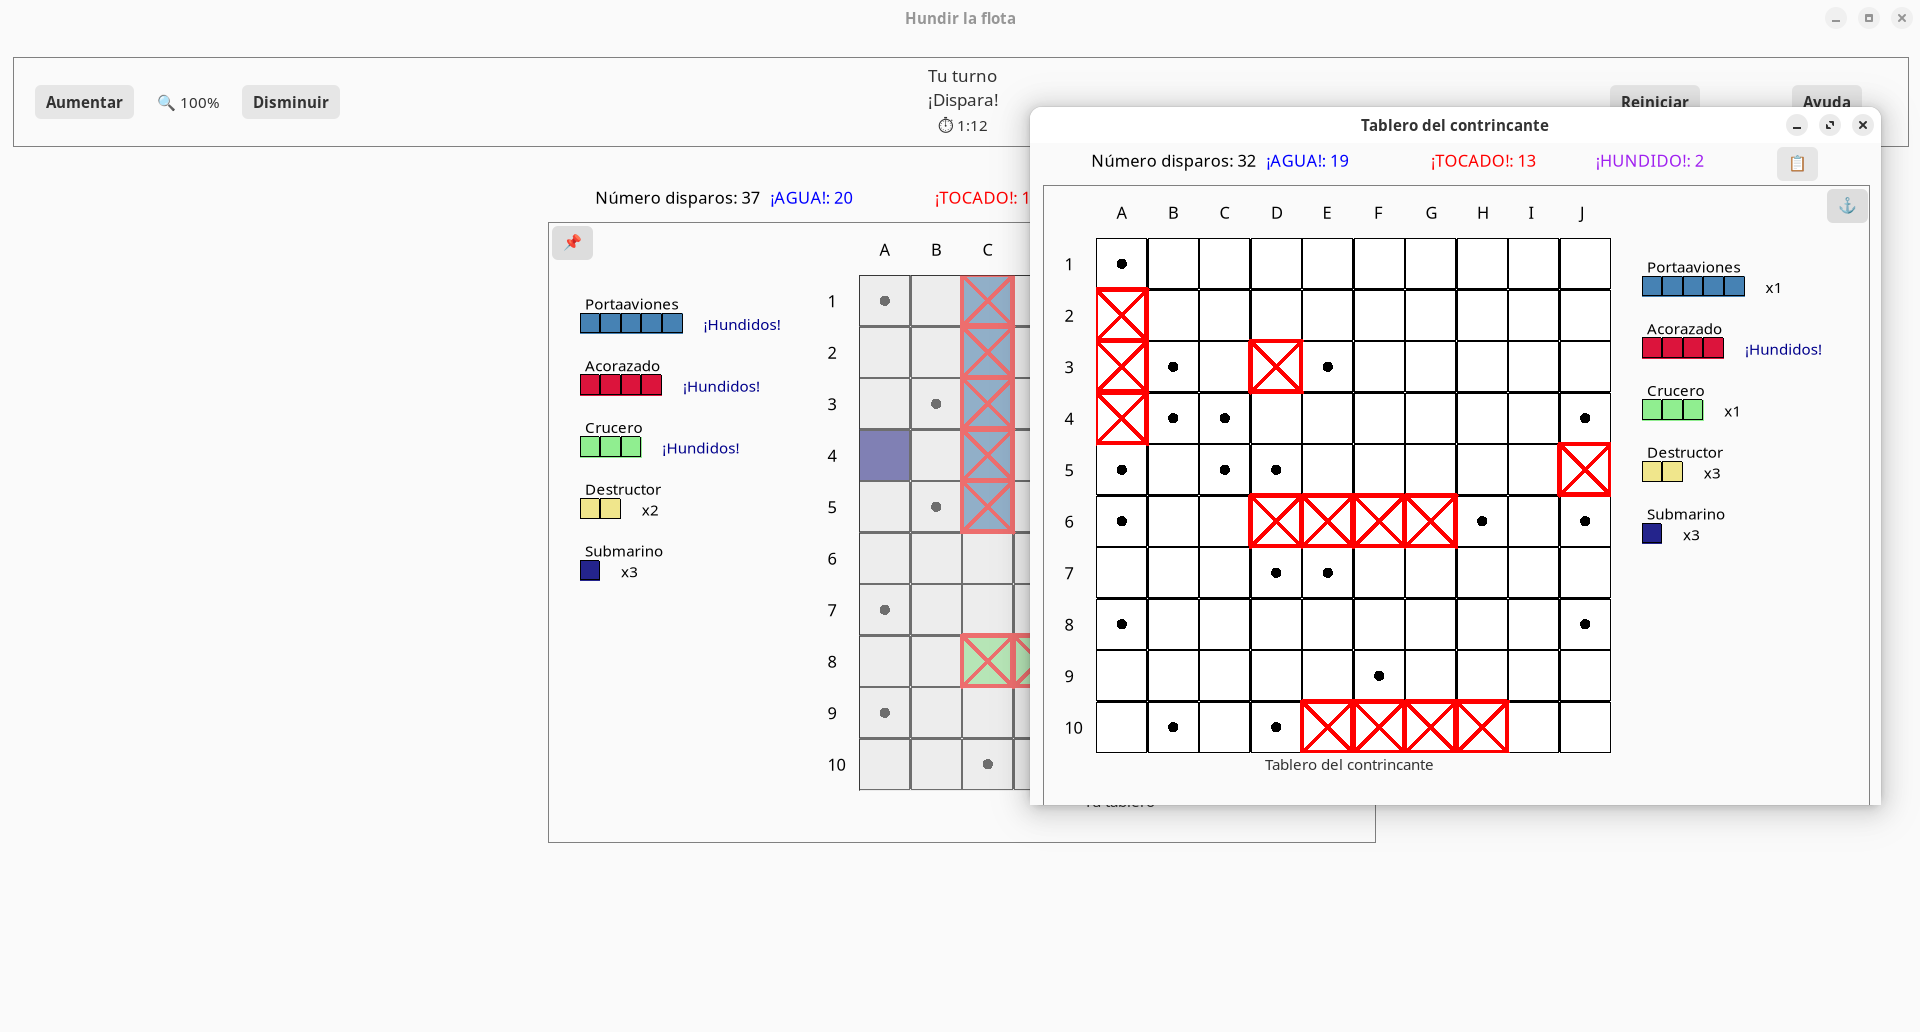
\includegraphics[width = \textwidth]{imagenes/resultados/desanclar.png}}
            \caption{Desanclar un tablero}
          \end{figure}
      \end{columns}
\end{frame}

\begin{frame}
    \begin{columns}
        \column{\dimexpr\paperwidth-10pt}
        \begin{figure}
            \scalebox{1}{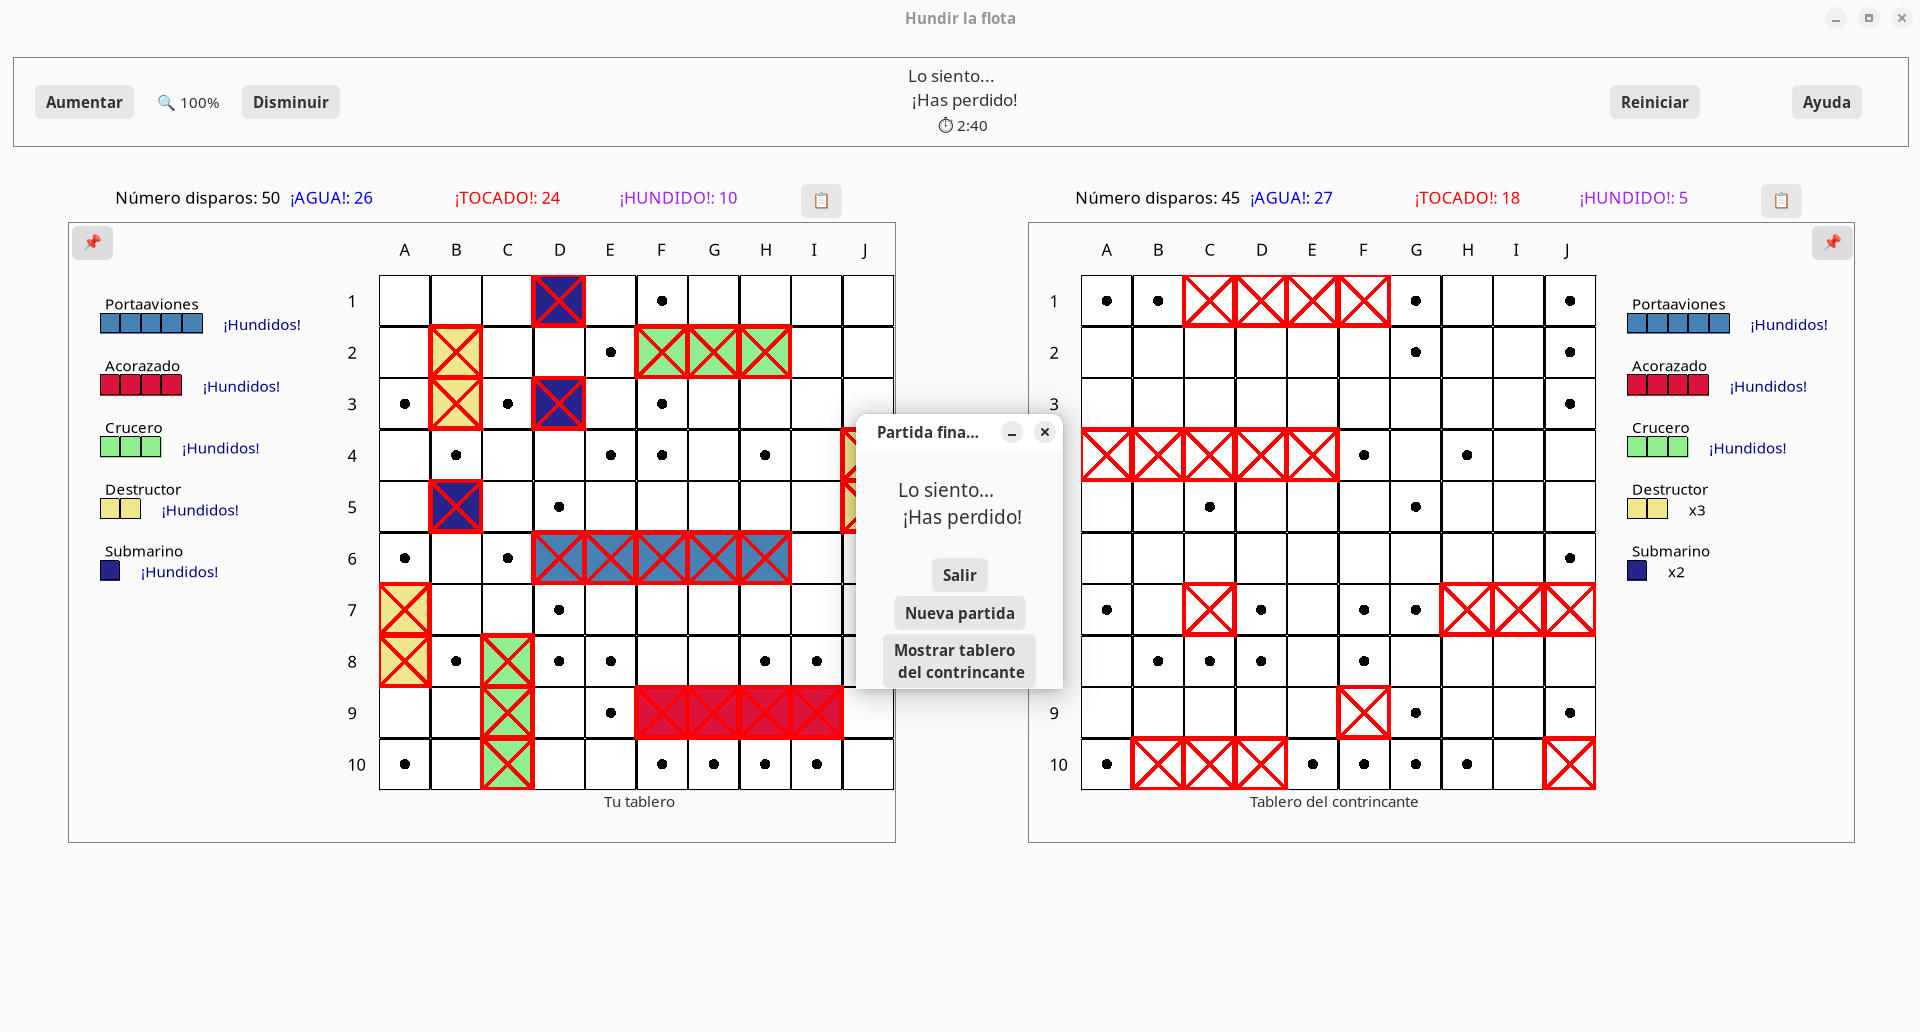
\includegraphics[width = \textwidth]{imagenes/resultados/final.png}}
            \caption{Final de una partida}
          \end{figure}
      \end{columns}
\end{frame}

\begin{frame}
    \begin{columns}
        \column{\dimexpr\paperwidth-10pt}
        \begin{figure}
            \scalebox{1}{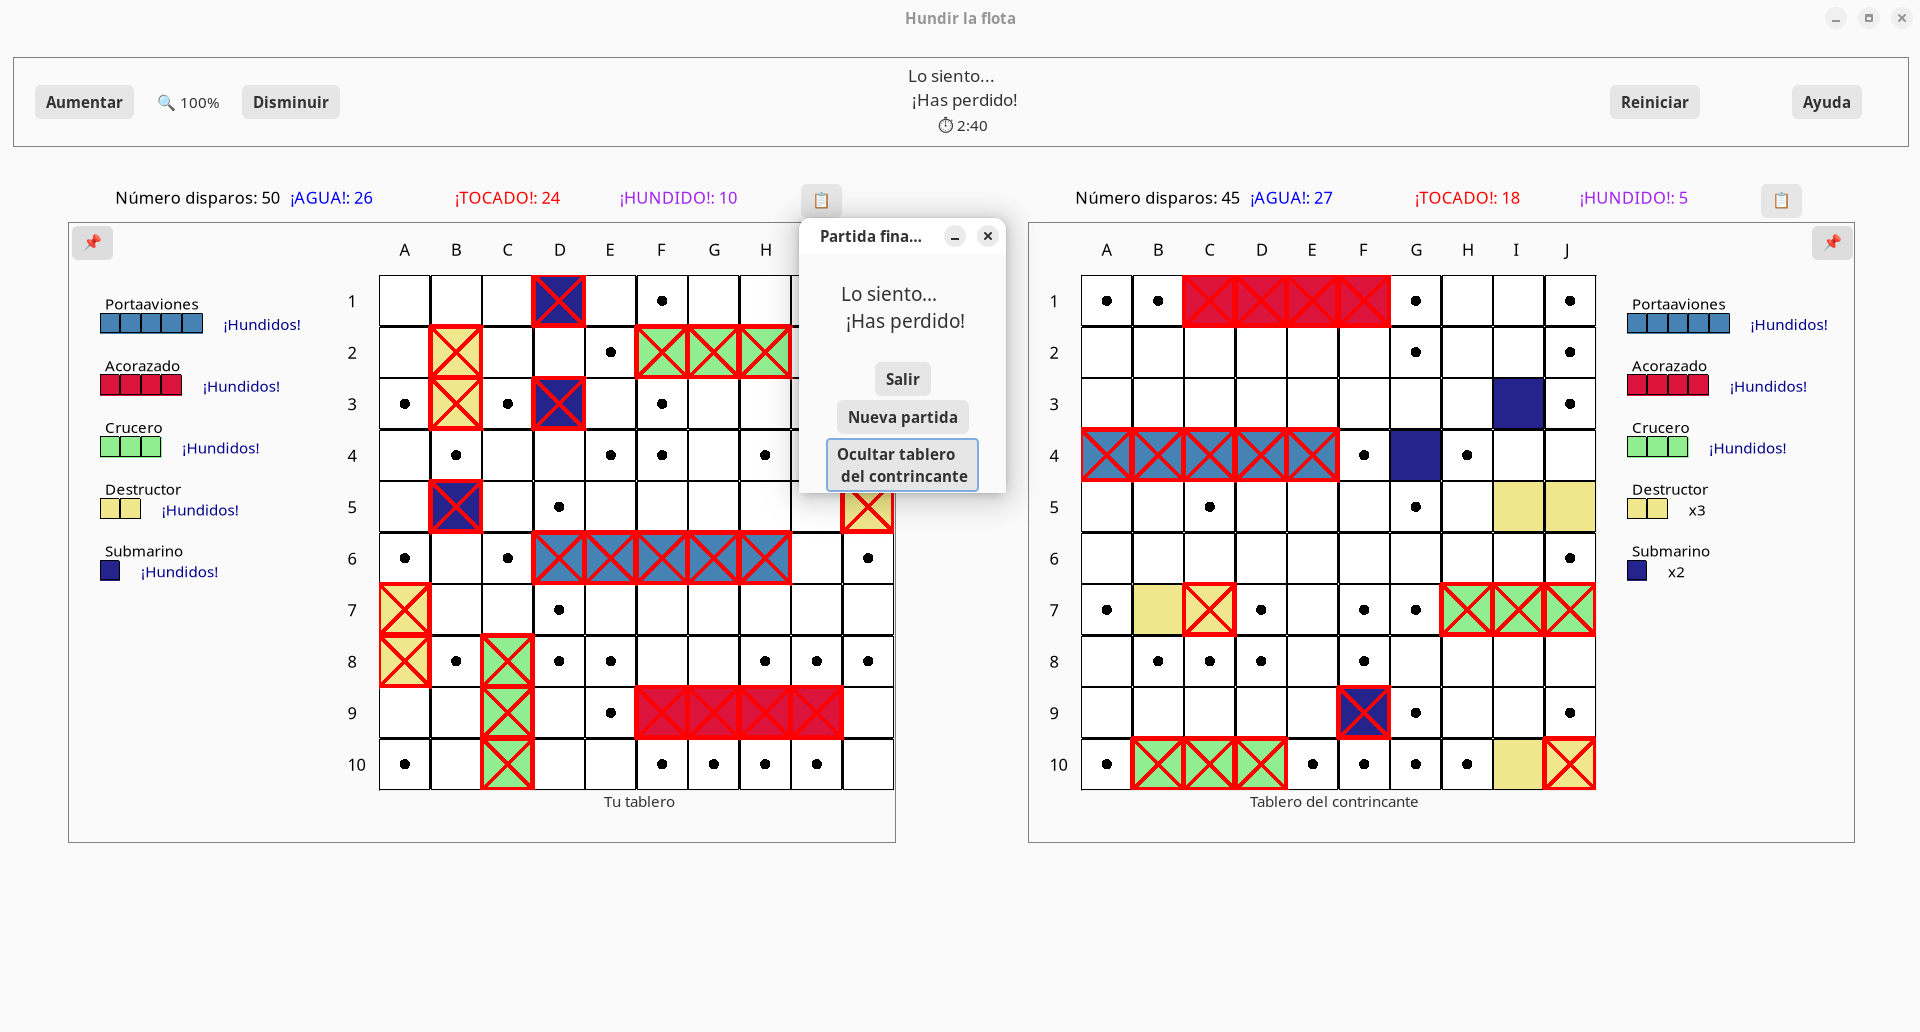
\includegraphics[width = \textwidth]{imagenes/resultados/mostrarTablero.png}}
            \caption{Mostrar el tablero de la CPU al finalizar}
          \end{figure}
      \end{columns}
\end{frame}

